\documentclass[../main.tex]{subfiles}
\graphicspath{{\subfix{../images/}}}

\begin{document}

\hypertarget{automatic-exploit-generation-module}{%
  \chapter{The Automatic Exploit Generation
    Module}\label{automatic-exploit-generation-module}}

The last module \cite{aeg_module_repo} given in this thesis aims towards automatic exploit generation.
It is directly linked to two modules to obtain the data it requires: the
vulnerability detection module, which provides proofs of vulnerabilities
(specifically, \texttt{ProofOfVulnerability} objects), and the vulnerability
analytics module, which provides further details about the exploitation
circumstances and exploitability.

\hypertarget{theoretical-aspects}{%
  \section{Theoretical Aspects}\label{theoretical-aspects}}

We investigated several articles on the subject to determine the current
academic development in the field of automatic exploit generation. All of them
can be classified as follows:

\begin{itemize}
  \tightlist
  \item
        Papers describing an automatic exploit generation (AEG) (sub)system \cite{aeg} \cite{mayhem_paper} \cite{bop} \cite{bof_aeg}:
        The majority of the studies examined handle the problem by combining
        it with vulnerability detection. In this manner, the systems discover
        software flaws by combining several methodologies and developing
        functional exploits.
  \item
        Papers summarizing the current AEG context \cite{crs_aeg_survey} \cite{alphahacking} \cite{code_reuse_survey}:
        This category does not show specific AEG system implementations, but
        rather examines methodologies and approaches proposed in functional
        cyber reasoning systems (for example, those from DARPA's Cyber Grand
        Challenge) and academia as separate exploitation research.
\end{itemize}

The following lists provide a summary of the most common flaws, mitigations,
(support) exploitation approaches, and consequences mentioned or used in the
studied papers:

\begin{landscape}
\vspace*{\fill}
\begin{figure}[!h]
   \centering
    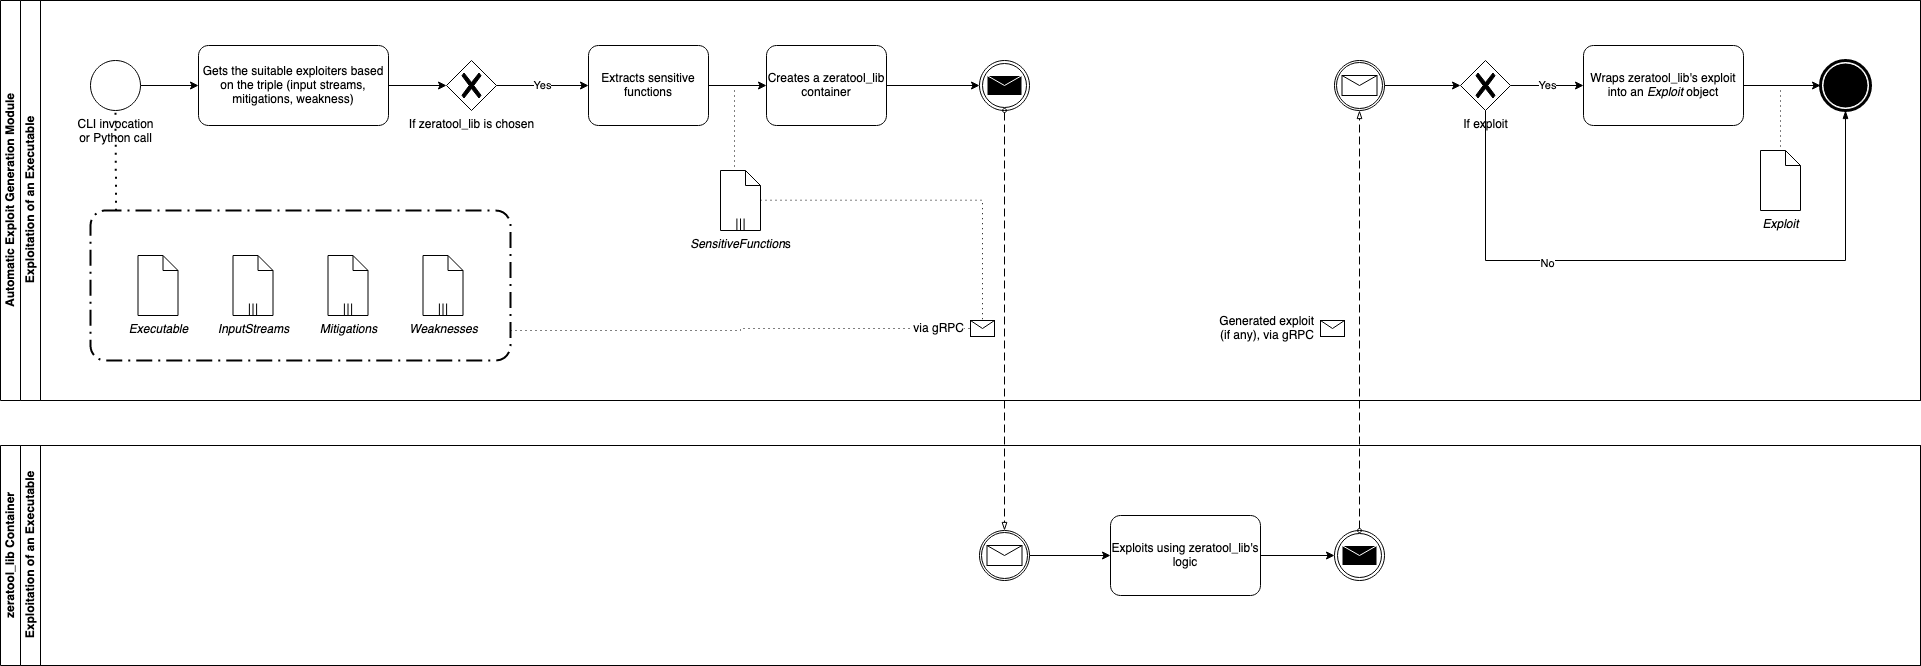
\includegraphics[width=0.95\linewidth]{images/aeg.png}
    \caption{Architecture of the Automatic Exploit Generation Module}
    \label{fig:vuln_architecture}
\end{figure}
\vspace*{\fill}
\end{landscape}

\begin{itemize}
  \tightlist
  \item
        Weaknesses

        \begin{itemize}
          \tightlist
          \item
                Out-of-bound memory writes: Consists of writing data whose length
                exceeds the buffer length. There are two types of allocation: on
                stack, for variables defined in a function, or heap, when the buffer
                is dynamically allocated. If the stack is targeted, then the return
                address and old base pointer can be overwritten.
          \item
                Type overflow: The correct result of an operation could not be
                stored in a certain type of variable.
          \item
                Tainted format strings: The first parameter of functions working
                with a format string (such as \texttt{printf}) is user controlled.
          \item
                Information leaks: The program divulges information about its
                execution (for example, memory layout).
        \end{itemize}
  \item
        Mitigations

        \begin{itemize}
          \tightlist
          \item
                Address Space Layout Randomization (ASLR): Segments such
                as the stack, dynamic libraries, and heap are placed randomly in the
                process memory space.
          \item
                Position Independent Execution: The code segment is placed, as in
                ASLR, randomly in the memory space. The program should be compiled
                with Position Independent Code enabled.
          \item
                NX bit: If enabled, the bit prevents a page to be executed and
                writable at the same time.
          \item
                Stack canaries: The canaries are values placed on the stack after
                entering a frame. It is checked on return and, if the check fails,
                then the execution is aborted.
          \item
                Control flow integrity: Permits only certain code, part of the valid
                control flow graph, to be executed. New code, injected by attackers
                in process memory, could not be executed anymore.
        \end{itemize}
  \item
        Exploitation techniques (including support ones)

        \begin{itemize}
          \tightlist
          \item
                Shellcode: Machine code is injected in process memory and executed
                by chaining with other techniques for hijacking the execution flow.
          \item
                Return-oriented programming (ROP): Unlike shellcodes, which inject new
                code, ROPs reuse code already existent in process memory. A chain of
                gadgets is created and executed by coupling the technique with
                execution flow hijack.
          \item
                Data-oriented programming (DOP): The accent in DOP resides on data flow
                and how it can be altered by using existent code constructs (similar
                to ROP).
          \item
                NOP sleds: This support technique is used with shellcodes to
                increase the probability that it will be executed correctly. The
                shellcode is prefixed with a \texttt{nop} sequence such that the
                execution could be redirected (for example, with return address
                overwrites) anywhere on the sled. This is in contrast to raw
                shellcode when the execution needs to start from the first shellcode
                byte.
        \end{itemize}
  \item
        Outcomes

        \begin{itemize}
          \tightlist
          \item
                Code execution: The programs execute the code desired by the
                attacker.
          \item
                Denial of service: The program functioning is blocked or halted at
                all.
          \item
                Information leaks: Sensitive information is extracted.
        \end{itemize}
\end{itemize}

\cite{bof_aeg} is an example of the whole data flow and operation of AEG
systems. It takes a similar approach to what we picked for our cyber
reasoning system. To begin, the proposed method obtains basic
information regarding active mitigations such as NX bits and ASLR. After
their mining module detects vulnerabilities, the protections are
circumvented via returns to system libraries in the case of NX bits and
\texttt{jmp\ esp} gadgets in the case of ASLR bypass. Then, a mathematical
solver is utilized to automatically construct an exploit while taking
the limitations into account. Binaries from the Cyber Grand Challenge
were used to validate the entire process.

For OpenCRS, we looked into open-source projects that already have exploitation
capabilities. Given our emphasis on 32-bit, C-based ELF executables, we came up
with two candidates:

\begin{enumerate}
  \def\labelenumi{\arabic{enumi}.}
  \item
        Ropstar \simplefootnote{https://github.com/xct/ropstar}: Given an executable that accepts file input and
        eventually has PIE, ASLR, NX, and canaries enabled, Ropstar attempts
        to launch a shell or call a sensitive (or "win"") function by
        exploiting buffer overflows and improper format string usage. It may
        utilize techniques such as \texttt{.got} and \texttt{.plt}
        overwriting, as well as return-oriented programming (with return to
        \texttt{libc} or \texttt{.plt}, or direct \texttt{setuid} and
        \texttt{system} calls) depending on the exploitation scenario. We
        choose to integrate the following sophisticated solution due to the
        limited input streams that are provided by default. It should be noted
        that we uncovered a command injection vulnerability during the code
        examination (to better understand the tool's internals), which we
        filed via a public issue \simplefootnote{https://github.com/xct/ropstar/issues/12} on GitHub. At the same time, a patch
        with a PR \simplefootnote{https://github.com/xct/ropstar/pull/11} was proposed, which had not yet been integrated by
        the repository maintainer at the time of writing this thesis.
  \item
        Zeratool \cite{zeratool}: The second open-source option we investigated (and
        integrated) is Zeratool, which is primarily used for CTF challenges.
        It is capable of exploiting stack-based out-of-bounds writes and
        format string weaknesses in binaries, although only the first has been
        included due to the prominence of the weakness in C-based executables.
        The exploits avoid eventual mitigations like as NX, PIE, and ASLR, and
        have the potential to:

        \begin{itemize}
          \tightlist
          \item
                Code execution

                \begin{itemize}
                  \tightlist
                  \item
                        Sensitive functions: Functions with names containing strings such
                        as "\emph{secret}", "\emph{shell}", and "\emph{system}", can
                        be called as functionality relevant to an attacker can be
                        unlocked;
                  \item
                        Shellcodes;
                  \item
                        Shell functions; and
                \end{itemize}
          \item
                Leaking data from memory, which can respect a Regex pattern that is
                set at the beginning of the exploitation.
        \end{itemize}
\end{enumerate}

\hypertarget{implementation}{%
  \section{Implementation}\label{implementation}}

OpenCRS modeled exploiters, which are independent exploitation logic capable of
generating exploits under specified parameters dictated by input streams,
mitigations, and results. These are validated by the method
\texttt{\_is\_exploitation\_supported}, which should be implemented in every
exploiter that derives from the \texttt{BaseExploiter} class.

In this manner, the automatic exploitation module can query all of its
exploiters to determine which can be used for a certain executable using an
exploiters manager. The attack surface approximation module already provides
the input streams and mitigations, and the results are specified in the CRS
configuration.

As previously stated, Zeratool was integrated into OpenCRS as an exploiter by
first forking the main repository \cite{zeratool_lib} into our organization's new
repository, \texttt{zeratool\_lib}. The original codebase was modified as
follows:

\begin{itemize}
  \tightlist
  \item
        The CLI was replaced with a unique function that CRS modules can call.
        As parameters of this function, all necessary parameters (input
        stream, method of exploitation, sensitive function, etc.) are
        accessible.
  \item
        Because of the local exploitation element of OpenCRS, all remote
        exploitation logic was removed.
  \item
        The main function returns the produced exploit.
  \item
        \texttt{libpwnable}, a library primarily used to aid with
        exploitation, is no longer an input stream. The only ones that are now
        supported are \texttt{stdin} and arguments.
\end{itemize}

If the query manager chooses Zeratool as a suitable exploiter for a certain
case, the sensitive functions are extracted. These are supplied together with
the binaries and its details through gRPC to a freshly built Docker container,
where a Python 3 service will unpack them and invoke \texttt{zeratool\_lib}. If
the exploitation procedure is successful, the exploit is read and wrapped into
a \texttt{Exploit} object.

\end{document}